\newpage
\section{Scaling applications}

\subsection{Introduction}

Scaling is a widely accepted measure of improving application performance leading to increase of offered Quality-of-Service. Enriching system with capability to scale entails avoiding additional costs that are related to coping with excessive traffic. In some cases, these costs may be caused by not handling extra traffic at all and may involve aspects such as: increased response time, processing overhead, space, memory, or money \cite{Bo00}. 

While scalability is a widely used term, it still lacks a clear and concise definition. Over the time, there were a few attempts to define it, yet not all of them were claimed as successful \cite{Hi90} \cite{DuRoWi06}. Hence, it is necessary to clarify this term before going into further discussion. Instinctively, scalability is perceived as an ability of a system to accommodate an increasing number of elements or objects to process. In particular, we can point out different types of scalability that are affected by increased number of requests: \cite{Bo00}:
\begin{itemize}
	\item \textit{load scalability} - an ability to work without delays and unproductive resource consumption at light, moderate, or heavy loads while making good use of available resources. Factors that may hinder load scalability include: scheduling shared resource, self-expansion, inadequate exploitation of parallelism
	\item \textit{space scalability} - memory requirements do not grow to intolerable levels as the number of items system supports increases
	\item \textit{space-time scalability} - system continues to function gracefully as the number of objects it encompasses increases by orders of magnitude
	\item \textit{structural scalability} - implementation or standards do not impede the growth of the number of objects system encompasses
\end{itemize}
Although, all of the aforementioned aspects are vital for any application, our work focuses solely on the first type of scalability. The reasoning behind this is that while all of these scalability types lies in direct responsibility of an application developer, the load scalability can be additionally improved by adding additional resources to a system. This brings us to a question what kind of resources are used by an application or more appropriately in context of this dissertation: \textit{what kind of resources can we add to improve application performance?} Required resources vary from application to application. However, among the most common one we can distinguish:
\begin{itemize}
	\item CPU
	\item memory
	\item storage
	\item network bandwidth
\end{itemize}

It is commonly agreed that there are two ways of adding a resource:
\begin{itemize}
	\item \textit{horizontal scaling (scaling out)} - adding more nodes to a system, such as servers in a context of distributed application
	\item \textit{vertical scaling (scaling up)} - increasing capacity of a single node in a system, i.e. adding additional memory, CPU, storage, etc.
\end{itemize}

Cloud computing makes scaling application especially interesting due to the illusion of a virtually infinite computing infrastructure \cite{VaRoBu11}. Virtualization technologies, which often underpins cloud computing platform, allows for resource manipulation in a dynamic, on-demand manner. Although cloud computing offers additional scaling capabilities, it increases solution complexity because it operates in different layers: server, platform and network as stated in \cite{VaRoBu11}. However, since platform containers are often represented either as virtual machines or another isolated environment (e.g. OpenShift leverages SELinux and cgroups) they are similar to server scaling and supports both scaling up and out. Therefore, the remaining of this chapter is focused solely on server scaling, omitting network scaling as it lays outside of scope of this dissertation.

Adding resources is only a part of the success - it should be accompanied by tuning application platform's configuration. For example, adding supplementary CPUs without increasing thread pool size makes a little sense. Similarly, in context of a Java application, we have to increase heap size, to make a good use of extra memory. While importance of application tuning cannot be underestimated, its detailed analysis lays outside of the scope of this dissertation. Figure \ref{fig:scalability-layers} presents different scalability layers and actions that can be taken at each level to improve application performance.

\begin{figure}[!ht]
  \begin{center}
    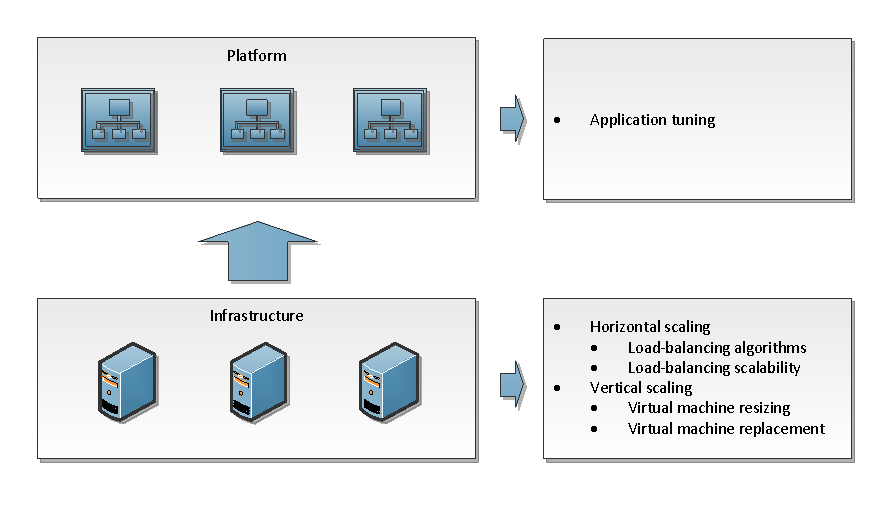
\includegraphics{chapter-scalability/scalability-layers}
  \end{center}
  \caption{Scalability layers}
  \label{fig:scalability-layers}
\end{figure}

With all that said, there is no silver bullet - not matter what underlying mechanism platform provider decides to use, the application developer is still responsible for creating an application with scaling in-mind. This statement has been already proven in 1967 by Amdahl law, which in short states that sequential component of a parallel algorithm impacts efficiency for a sufficiently large number processors \cite{Am67} as shown in Figure \ref{fig:amdahl-law}. In other words, adding supplementary resources to a poorly written application (i.e. having a lot of sequential or synchronized components) can be beneficial only to a certain degree. 

\begin{figure}[!ht]
  \begin{center}
    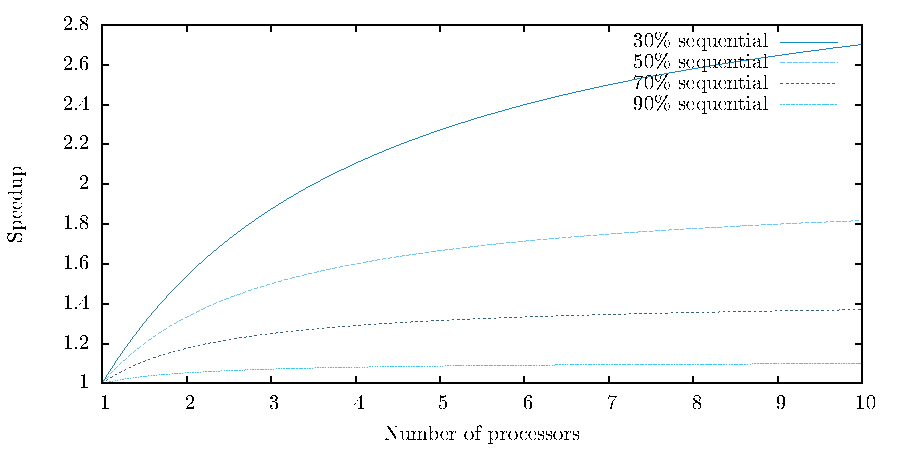
\includegraphics{chapter-scalability/amdahl-law}
  \end{center}
  \caption{Amdahl's law}
  \label{fig:amdahl-law}
\end{figure}

The rest of this chapter elaborates in detail about horizontal and vertical scaling taking into account mechanisms used in Platform-as-a-Service solutions that are available on the market.

\subsection{Horizontal scaling}
As outlined in previous section, horizontal scaling is about adding supplementary nodes to a system. In cloud computing, it is common to represent nodes as virtual machines and this assumption is used in further discussion. Consequently, adding server comes down to cloning a new virtual machine from a template and possibly installing additional software and reconfiguring it later. While mechanism of creating new virtual machine from a template is offered literally in every IaaS platform currently available (OpenStack \cite{OpenStack}, OpenNebula \cite{OpenNebula}, CloudStack \cite{CloudStack} or Eucalyptus \cite{Eucalyptus} to name a few) and is similar in manner, the underlying hardware and virtualization mechanism determines how fast provisioning is done. 

Provisioning new server is only a first step in scaling an application, it is required to configure load balancing mechanism to make use of additional node. The two important aspects that have to be consider are: load-balancing algorithms and load-balancing scalability.

\subsubsection{Load-balancing algorithms}
Generally, there are two types of load-balancers: hardware and software based. Due to the dynamic nature of application requirements, we focus only on the latter as it offers a greater deal of flexibility. Among the most common algorithms we can distinguish \cite{HaProxyDoc}:
\begin{itemize}
 \item \textit{round-robin scheduling} - request are sent to successive nodes, according to their weights. This algorithm is fairest when processing time remains equally distributed \cite{HaProxyDoc}
 \item \textit{least connection} - the server with the lowest number of connections receives the connection
 \item \textit{source routing} - source IP address is hashed, the same client IP address always reaches the same server
 \item \textit{URI hashing} - URI that designates resource is hashed and divided by the total weight of the running servers. Such hash designates which server receives the request. In practice, this algorithm is commonly used with proxy caches and anti-virus proxies in order to maximize the cache hit rate.
 \item \textit{request counting algorithm} - load is distributed the requests among the various workers, ensuring that each gets its configured share of the number of requests
 \item \textit{weighted traffic counting algorithm} - variation of the above-mentioned algorithm. However, it is focused on bytes rather than number of request
 \item \textit{pending request counting algorithm} - scheduler keeps track of how many requests is assigned to each worker. A new request is automatically assigned to the worker with the lowest number of active requests
\end{itemize}

Situation gets further complicated when considering real-world web application that sends user information using cookies, what imposes on load-balancer requirement for session stickiness \cite{StBaMa11}. 

\subsubsection{Load-balancing scalability}
Although, it may seem that balancing workloads eliminates problem of a single point of failure (SPOF) among different servers, it is in fact shifted to load-balancing layer. In other words, load-balancer becomes a new SPOF. Therefore, in cases where high availability is required, multi-tiered load balancing architecture should be considered. This, however, seems not to be a case among current IaaS or PaaS providers - none of them unequivocally specifies whether their provide redundancy at load-balancer level.

\subsubsection{Load-balancer comparision}

While there are many load-balancers available on the market, following are credited to be the most popular:
\begin{itemize}
 \item \textbf{HAProxy} \cite{HAProxy} - load-balancer initially written by Willy Tarreau. Noticeably, it's used by OpenShift \cite{OpenShift} to distribute load among gears \cite{OpenShiftScaling}
 \item \textbf{BIG-IP Local Traffic Manager (LTM)} - solution offered by F5 \cite{F5}. Although LTM is a hardware solution, omitted in this section, it also has its virtualized counterpart.
 \item \textbf{Apache HTTPD} \cite{ApacheHTTPD} - popular HTTP server. When enhanced with additional modules, it can behave like a proxy or load-balancer. Over the time, there were several attempts to develop such modules: mod\_jk \cite{ApacheModJk}, mod\_proxy\_balancer \cite{ApacheModProxyBalancer}, to name a few. While the former is purely AJP13 oriented, the latter supports different protocols: HTTP, FTP and AJP13. As a consequence, only mod\_proxy\_balancer was taken into account during comparision. 
 \item \textbf{Zeus Load Balancer} \cite{Zeus} - load balancer offered by layer47 \cite{Layer47}, it incorporates techniques such as Layer-7 traffic management and content aware algorithms
 \item \textbf{Zeus Global Load Balancer} \cite{ZeusGlobal} - load balancer offered by layer47 \cite{Layer47}, it is specialised in balancing load among globally distributed data centres
 
\end{itemize}

Table \ref{tab:load-balancer-comparison} presents they key performance features and algorithm used to schedule requests.

\begin{table}[!htbp]
\begin{tabularx}{\textwidth}[]{ X  X  X }
\specialrule{.1em}{.05em}{.05em} 

  & \textbf{Performance features} & \textbf{Scheduling algorithms} \\
\specialrule{.1em}{.05em}{.05em} 

HAProxy \cite{HAProxy} & 
-- a single-process, event-driven model reduces the cost of context switch and the memory usage
 
-- O(1) event checker
 
-- single-buffering without copying data between reads and writes
 
-- zero-copy forwarding
 
-- optimized HTTP header analysis: headers are parsed and interpreted on the fly
 
&
-- round-robin scheduling

-- least connection

-- source routing

-- URI hashing
\\ \hline

BIG-IP Local Traffic Manager \cite{LTM} &
-- managing application services level rather than individual devices and objects

-- scripting language that allows administrator to intercept, inspect, transform, and direct application traffic

-- built-in firewall protection, application security, and access control

-- real-time protocol and traffic management decisions
& 

\\ \hline

Apache HTTPD \cite{ApacheHTTPD} & 
-- support for session stickiness by using cookies and URL encoding. This approach \cite{ApacheModProxyBalancer} avoids unequal load distribution if clients are hidden behind proxies and stickyness errors when a client uses a dynamic IP address that changes during a session
& 
-- request counting algorithm

-- weighted traffic counting algorithm

-- pending request counting algorithm
\\ \hline

Zeus Load Balancer \cite{Zeus} & 

-- Layer-7 traffic management

-- HTTP content compression

-- connection concurrency control

-- server health monitoring

& 
-- content-aware algorithms
\\ \hline

Zeus Global Load Balancer \cite{ZeusGlobal} & 

-- service health monitoring

-- active - passive failover

-- balancing is based on observed performance

& 
-- geographic proximity

-- adaptive load balancing (based on proximity and load)

\\ \hline

\end{tabularx}

\caption{Comparison of load balancers}
\label{tab:load-balancer-comparison}

\end{table}

\newpage
\subsection{Vertical scaling}
Essentially, vertical scaling is concentrated upon increasing capacity of a single node. Again, when considering technical advancements that comes with cloud computing and virtualization, we can differ two categories of scaling: virtual machine resizing and virtual machines replacement. This distinction is dictated by limitation of hypervisors - not all of them are able to resize virtual machine without shutting it down.

\subsubsection{Virtual machine resizing}


\begin{table}[!htbp]
\begin{tabularx}{\textwidth}{ l  X  X  X }
\specialrule{.1em}{.05em}{.05em} 
 & \textbf{Memory} & \textbf{CPU} & \textbf{Disk} \\
\specialrule{.1em}{.05em}{.05em} 

KVM 1.2.0 &
  & 
-- dynamic pinning CPU to a specific virtual machine (depending on underlying hardware)
& 
-- adding a disk to a LVM group

\\ \hline
Xen 4.3 & 
-- changing the amount of host physical memory assigned to virtual machine without rebooting it

-- start additional virtual machines on a host whose physical memory is currently full, by automatically reducing the memory allocations of existing virtual machines in order to make space
&
-- dynamic pinning CPU to a specific virtual machine (depending on underlying hardware)
&
-- dynamic block attaching, adding a disk to a LVM group

\\ \hline
VMware ESX 5.1 &
-- hot-plugging memory, ex. using VMware vSphere
&
-- hot-plugging CPU, ex. using VMware vSphere
&
-- adding additional disks to existing virtual machine

\\ \hline
OpenVZ (kernel: 042) &
-- configurable via user beancounters
&
-- configurable via user beancounters 
& 
-- configurable via user beancounters
\\ \hline
\end{tabularx}
\caption{Comparison of hypervisors resizing capabilities}
\label{tab:hypervisors-resizing}
\end{table}


\subsubsection{Virtual machine replacement}
As it was highlighted in previous section, reasoning behind virtual machine replacement is that, in case when dynamic resizing is not possible, a new virtual machine with a desired configuration can be provisioned and replace the old one. This is a basic operation and therefore all above-mentioned hypervisors support it as long as required resources are available. 

